\begin{figure*}[!h]
\begin{subfigure}{0.24\linewidth}
\centering
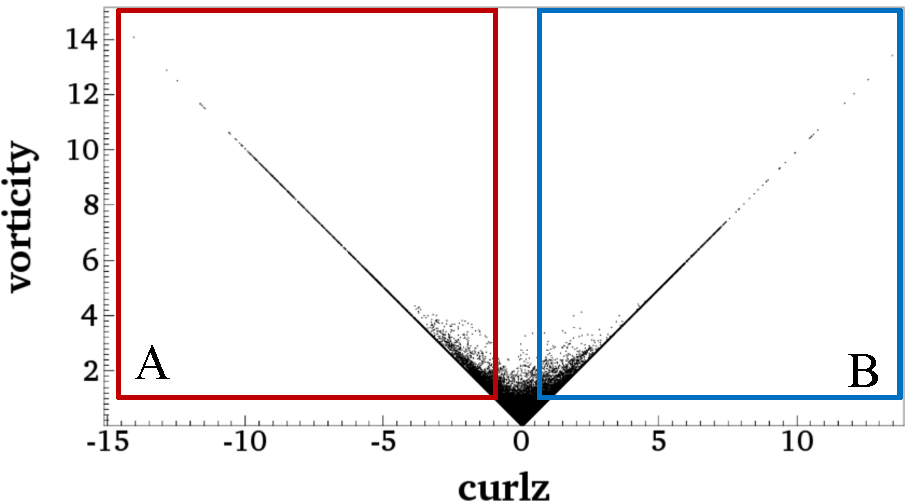
\includegraphics[width=0.95\linewidth]{Images/RedSeaEddy/scatterplot.pdf}
\vspace{-2mm}
\caption{2D scatterplot of $\mathcal{A}$ and traits. We use $T = \left\{T_{A}, T_{B}\right\}$.} 
\label{fig:rse_scatterplot}
\end{subfigure}
\hfill
\begin{subfigure}{0.245\linewidth}
\centering
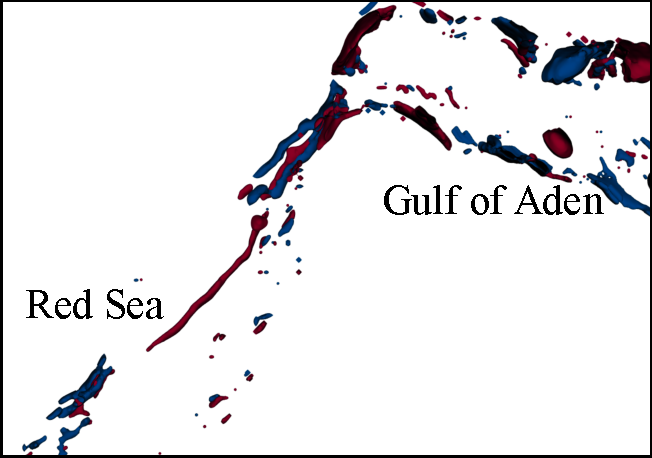
\includegraphics[width=\linewidth]{Images/RedSeaEddy/zls.pdf}
\vspace{-3mm}
\caption{$ZLS_{T}$}
\label{fig:rse_zls}
\end{subfigure}
\begin{subfigure}{0.245\linewidth}
\centering
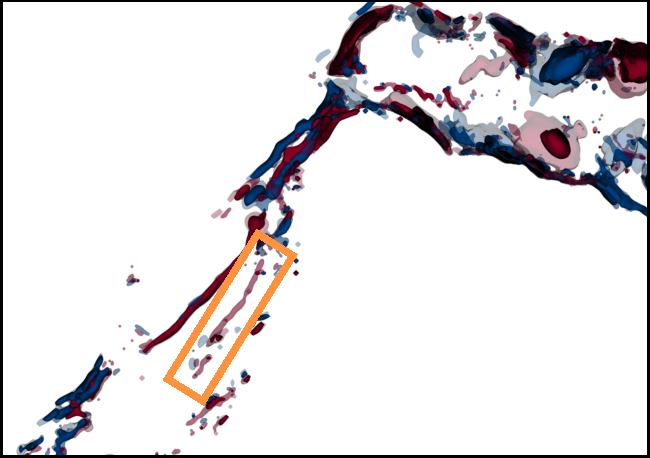
\includegraphics[width=\linewidth]{Images/RedSeaEddy/fcls_50.pdf}
\vspace{-3mm}
\caption{+ $FCLS_{T,50\%}$}
\label{fig:rse_fls}
\end{subfigure}
\begin{subfigure}{0.245\linewidth}
\centering
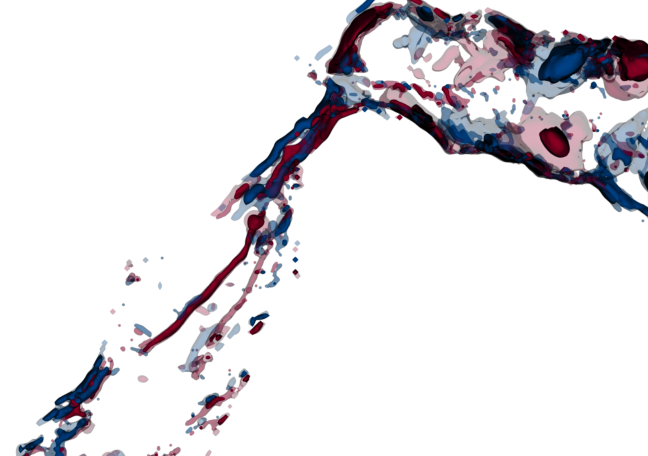
\includegraphics[width=\linewidth]{Images/RedSeaEddy/fcls_68.pdf}
\vspace{-3mm}
\caption{+ $FCLS_{T,68\%}$}
\label{fig:rse_fcls}
\end{subfigure}
\vspace{-2mm}
\caption{Visualization of anticyclonic~($T_{A}$, red) and cyclonic~($T_{B}$, blue) eddies in the Gulf of Aden and part of the Red Sea using the derived attributes of vorticity magnitude and the z-component of curl. For this ensemble data set~\cite{sanikommu2020impact}, the uncertainty resulted in $FCLS_{T,C}$ visualizing additional paths and regions with eddies. The orange boxes in (b) and (c) highlight one such example.}
\label{fig:rse}
\end{figure*}
